\subsection{Model-complexity and model-selection}


In this section we try to compare the performances of the Perceptron, we implemened during the first assignment against the SVM from this one.
Since the Perceptron can only handle linearly separable data, we will use a SVM with hard margin and linear Kernel for this comparison.
\\
\\
To select a proper test set we selected $M = 150$ training sets $\tau _{k},k \in \{1,\ldots,M\}$ form the MNIST training set with no more than $N = 70$ images each.
For $k \in \{1,\ldots,M\}$ we trained both SVM and Perceptron using $\tau_k$ and calculated the test error rate $R_k = \sum_{i=1}^{n}( (t_{i}^{\ast} - \hat{t_{i}} )^2 * \frac{1}{4n} ) $ on the {MNIST} test set - again for both SVM and Perceptron.
\\
\\
The average error $R_{avg} = \frac{1}{M}\sum_{k=1}^M R_k$ of SVM and Perceptron can be seen in the table below (Table \ref{tab:avg_error}).
Figure \ref{fig:error_SVM_perc} shows $\tau_k$ with the error rate for $\tau_k$.\\
As we can see in figure \ref{fig:error_SVM_perc_boxplot} the SVM has a more stable detection rate.

%As we can see performs the SVM already better than the Perceptrom, which still has to be verified.
%Against our expectations SVM does not perform as well as suspected, which could be due to the use of the linear Kernel and $C=\infty$ (no slack variables).
%Otherwise we would have suspeceted the SVM would have found a decision boundary similar or better than Perceptron.

\begin{table}[!h]
 \begin{center}
\begin{tabular}{|c|c|}
 \hline
 \textbf{$R_{avg}$ SVM} & \textbf{ $R_{avg}$ Perceptron} \\
 \hline
 0.014408163265306124       &     0.02609523809523809      \\
 \hline
  \hline
 \textbf{$R_{max}$ SVM} & \textbf{ $R_{max}$ Perceptron} \\
 \hline
0.04081632653061229       &     0.14540816326530615      \\
 \hline
\end{tabular}
\caption{\label{tab:avg_error} $R_{avg}$ for both algorithms }
\end{center}
\end{table}

\begin{figure}[!h]
\begin{center}
\centering
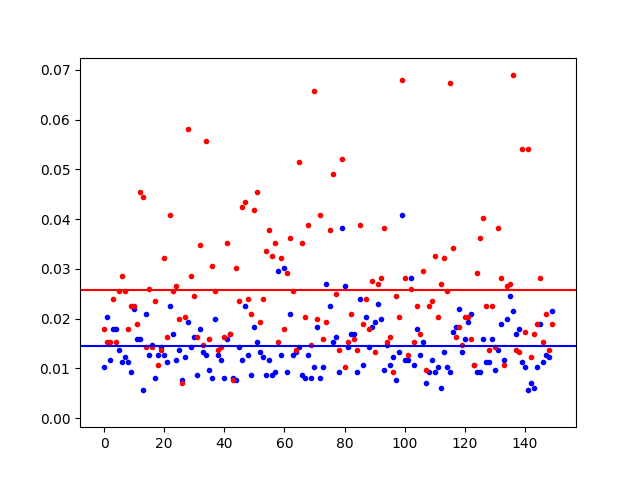
\includegraphics[width=1\textwidth]{figures/new/perc_vs_svm}
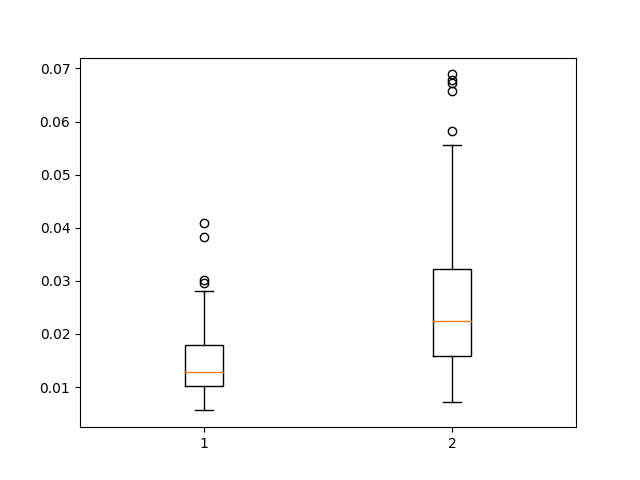
\includegraphics[width=1\textwidth]{figures/new/perc_vs_svm_boxplot}
\end{center}
\caption{\label{fig:error_SVM_perc} Comparing the error rates of $\tau_k$ from SVM (blue/1 ) against Perceptron(red/2) }
\end{figure}



\subsection{Tuning meta-parameters $C$ and $\sigma$}

This last section describes the effects of changing $C$ and $\sigma$ when using a RBF-kernel. In general $C$, a slack varibale, allows to not meet the margin requirement at a cost proportional to a value, which still allows us to minimize the error, but relaxes the stiffnes of linear separability.


To get a better understanding we took 135 sets from the MNIST training set with 35 images for training using varying values fo $C$ and $\sigma$ respectively and testing against the the MNIST Test data set with 10k images. $C$ is in the range ${5, 10, 15}$ $sigma$ is in ${4, 24, 50}$ and all of those combinations are used to train the SVM and calculate the average error for over the 135 training samples. 
Figure \ref{fig:3_1} shows a scatter plot of the average training error versus the  test error, which let us to the conclusion that there is direct  relation between training and test error. High training errors will lead to high test errors.\\

\begin{figure}[!h]
\begin{center}
\centering
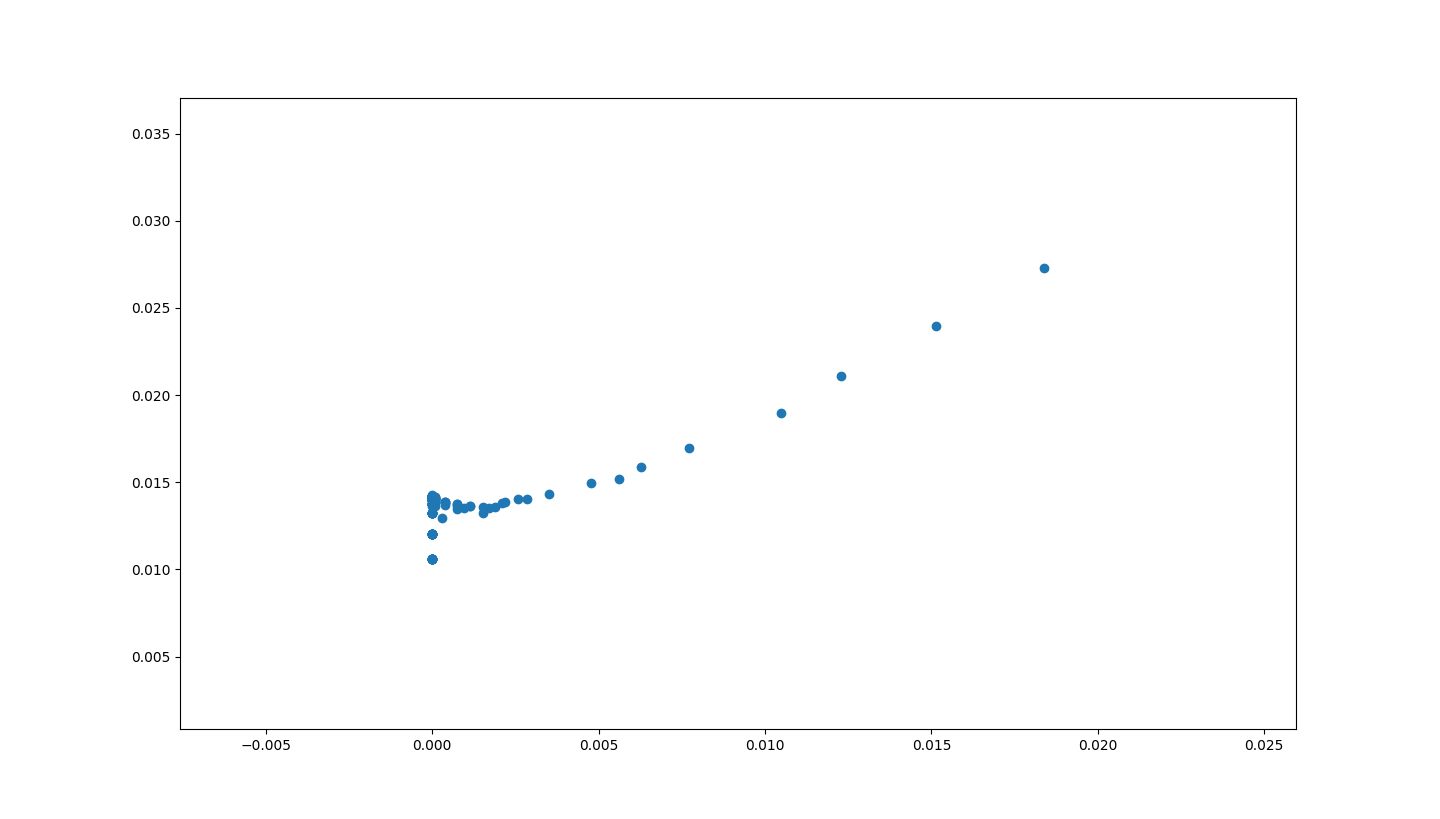
\includegraphics[width=1\textwidth]{figures/new/3_Figure_1}
\end{center}
\caption{\label{fig:3_1}  Test error in relation to the Training error  }
\end{figure}


Another metric we captured during our test runs was the number of support vectors. Figure \ref{fig:3_2} puts this number in relation to the average test error.  Here we can see multiple insights. 

First, most of the test runs yielded less than $40$ support vectors, with the number of such ranging from $25$ to $53$. The data points are more dense on the left side of the range.\\
Secondly there is a visible correlation between the number of support vectors and the test error, when you ignore some outliers. However it seems that the sweet spot is located at 27 instead of 25, since there is a little drop in the observed error rate shortly after the beginning (at 25 ), which then rises again steadily to reach the maximum at location 53.


\begin{figure}[!h]
\begin{center}
\centering
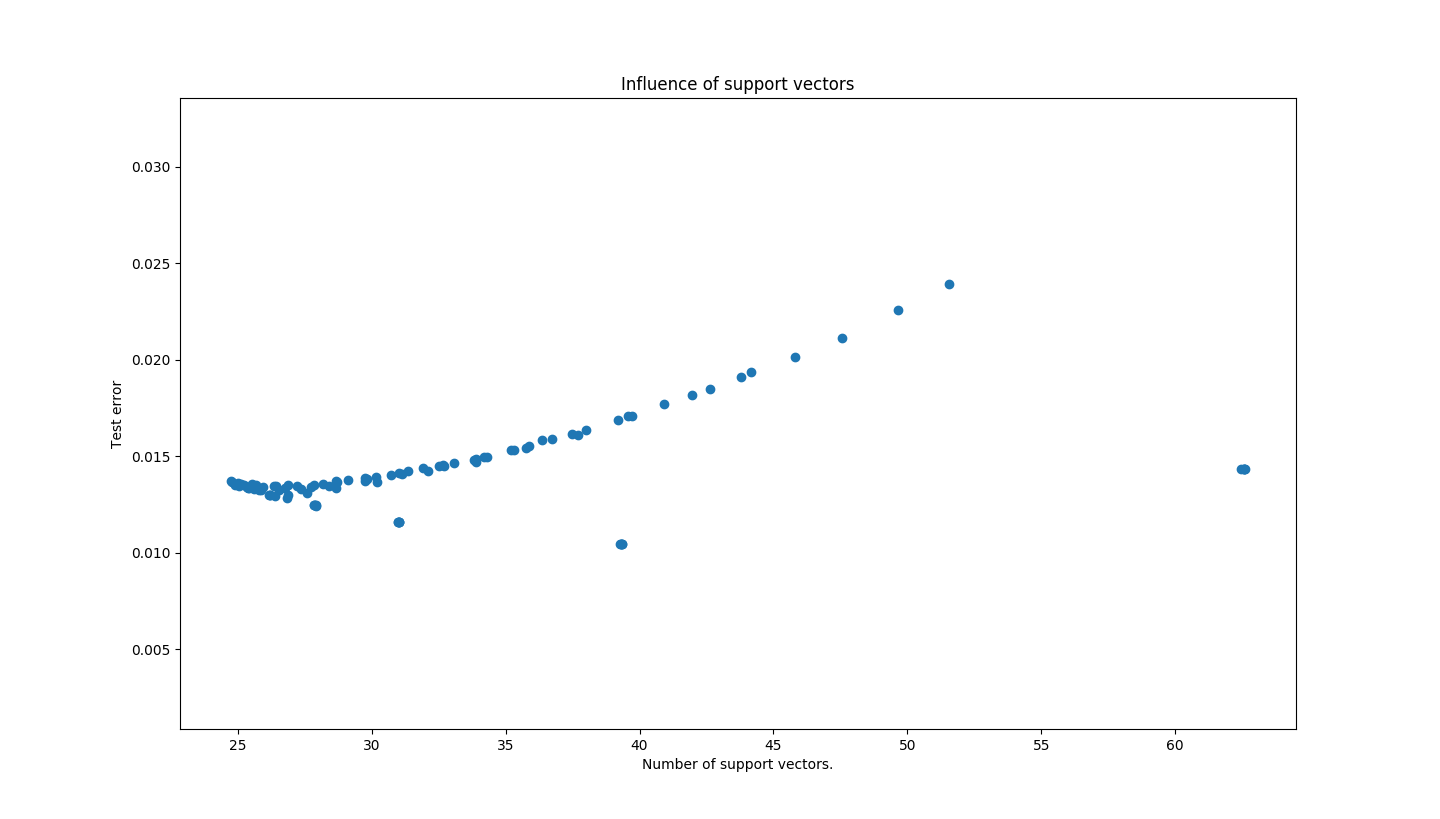
\includegraphics[width=1\textwidth]{figures/new/3_Figure_2}
\end{center}
\caption{\label{fig:3_2} Number of support vectors in relation to the test error}
\end{figure}


\subsection{Finding the best $C$ and $\sigma$}

Figure \ref{fig:3_3} and \ref{fig:3_4} show us the relation between varying values for $C$ and $\sigma$ and the average training and testing error. Both images hold the same information, but in different representation. We can see that low values for $C$ and high values $\sigma$  result in worse detection rates. 
During our runs with $M$-fold cross validation we found the best suitable combination to be 
\begin{align*}
C= 25.454545454545453\\
\sigma=8.181818181818182 \\
\text{with an average error of } 0.013124320869287314
\end{align*}
These values align very well with the parameter space we during our experiments, see figure \ref{fig:3_4}. When comparing the results for our best performing RBF SVM against a linear SVM (see table \ref{tab:results}), we can see that our champion RBF SVM outperforms the linear SVM by 0.318 \% on average.

\begin{table}[!h]
 \begin{center}
\begin{tabular}{|l|l|l|}
 \hline
 & \textbf{RBF SVM} & \textbf{linear SVM} \\
 \hline
  \textbf{$R_{whole Set}$} & 0.0020408163265306367       &     0.004081632653061273      \\
 \hline
  \hline
 \textbf{$R_{avg}$} & 0.011227891156462583       &     0.014408163265306122      \\
 \hline
 \textbf{$R_{min}$} & 0.004081632653061273       &     0.0056122448979591955      \\
 \hline
  \textbf{$R_{max}$} & 0.03367346938775506       &     0.04081632653061229      \\
 \hline
 
\end{tabular}
\caption{\label{tab:results} comparing RBF SVM with best parameters to linear SVM }
\end{center}
\end{table}



\begin{figure}[!h]
\begin{center}
\centering
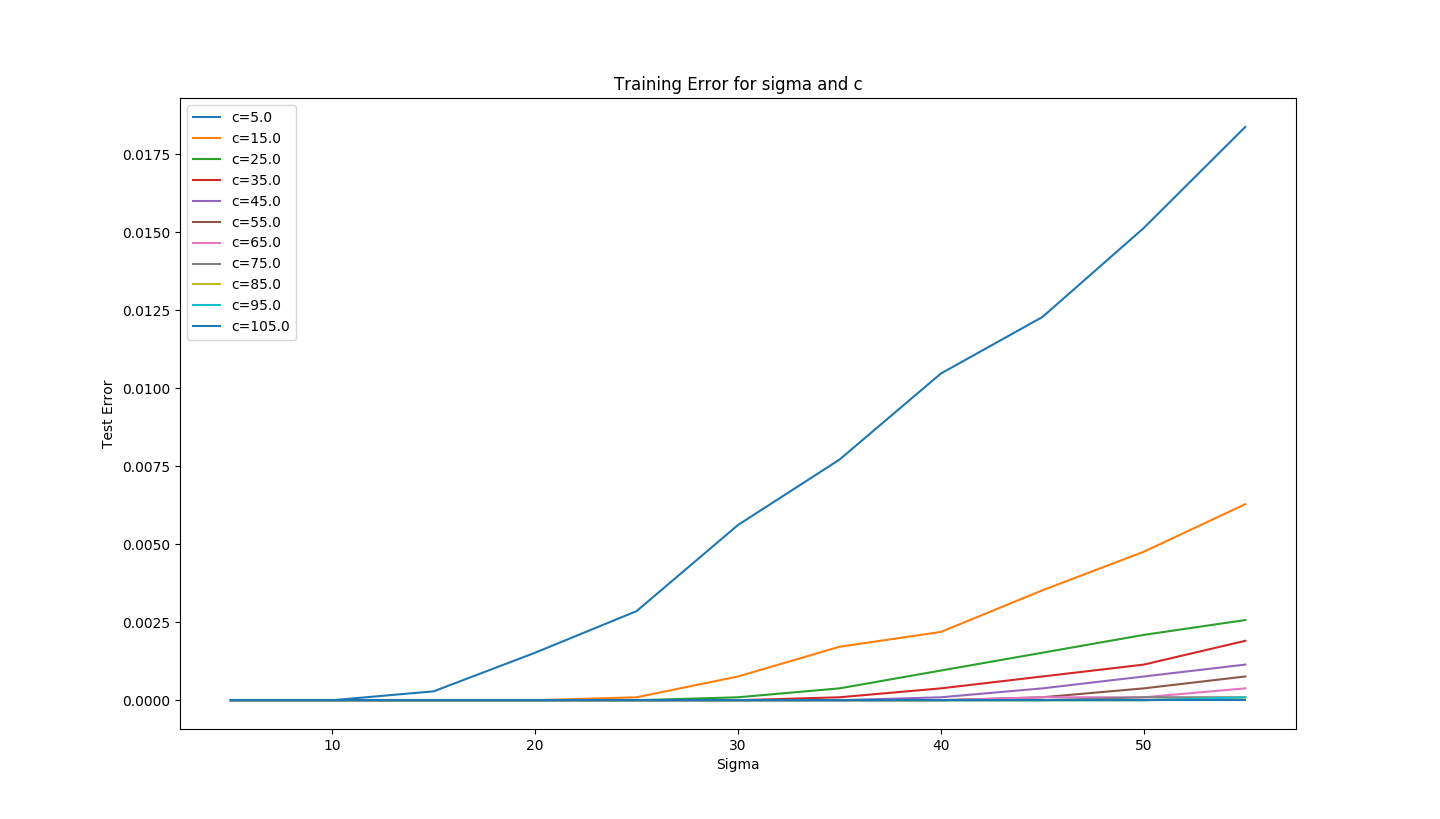
\includegraphics[width=1\textwidth]{figures/new/3_Figure_4}
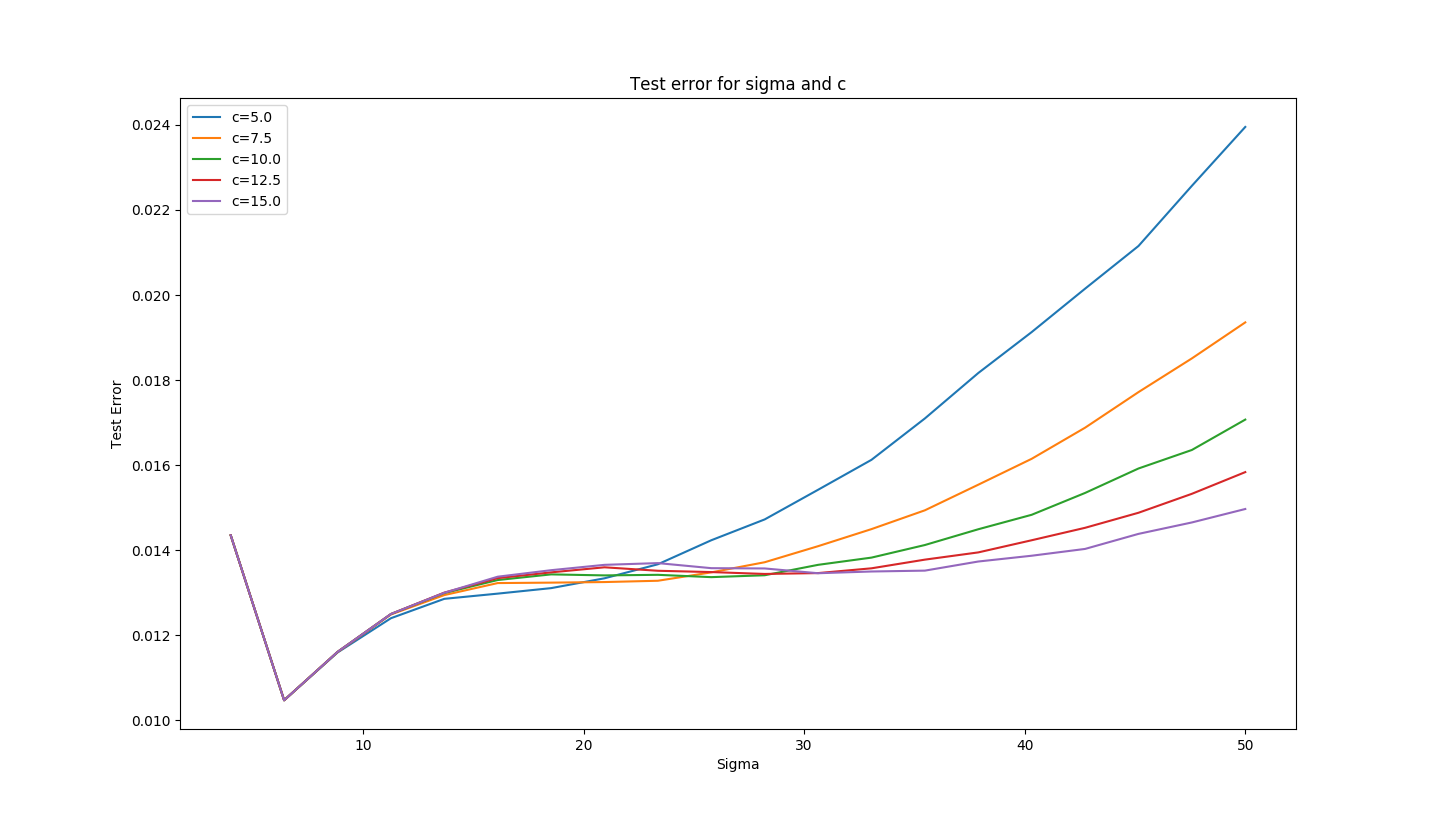
\includegraphics[width=1\textwidth]{figures/new/3_Figure_3}
\end{center}
\caption{\label{fig:3_3} Impact of varying values of $C$ and $\sigma$ on training and test error  }
\end{figure}

\begin{figure}[!h]
\begin{center}
\centering
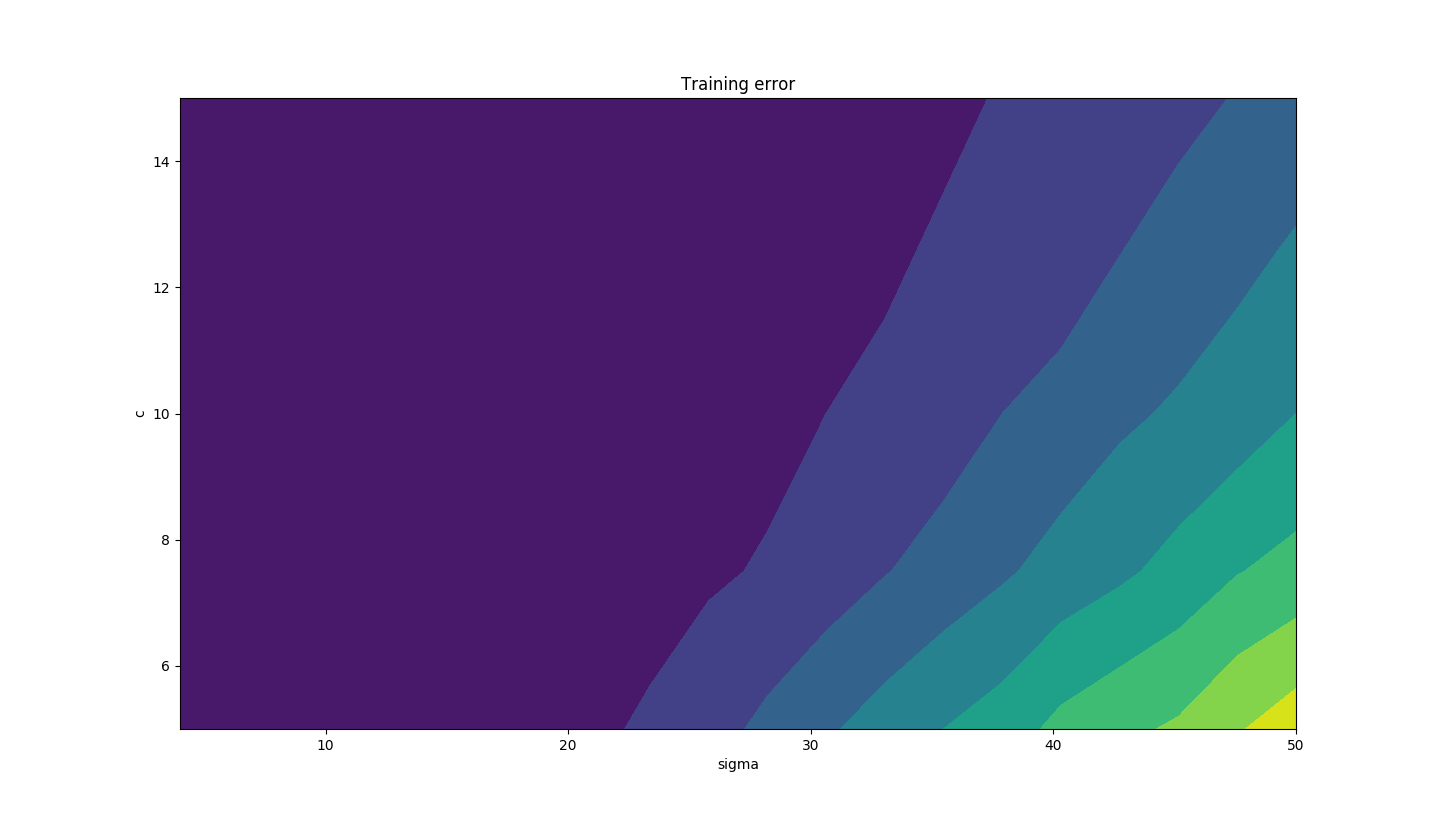
\includegraphics[width=1\textwidth]{figures/new/3_Figure_6}
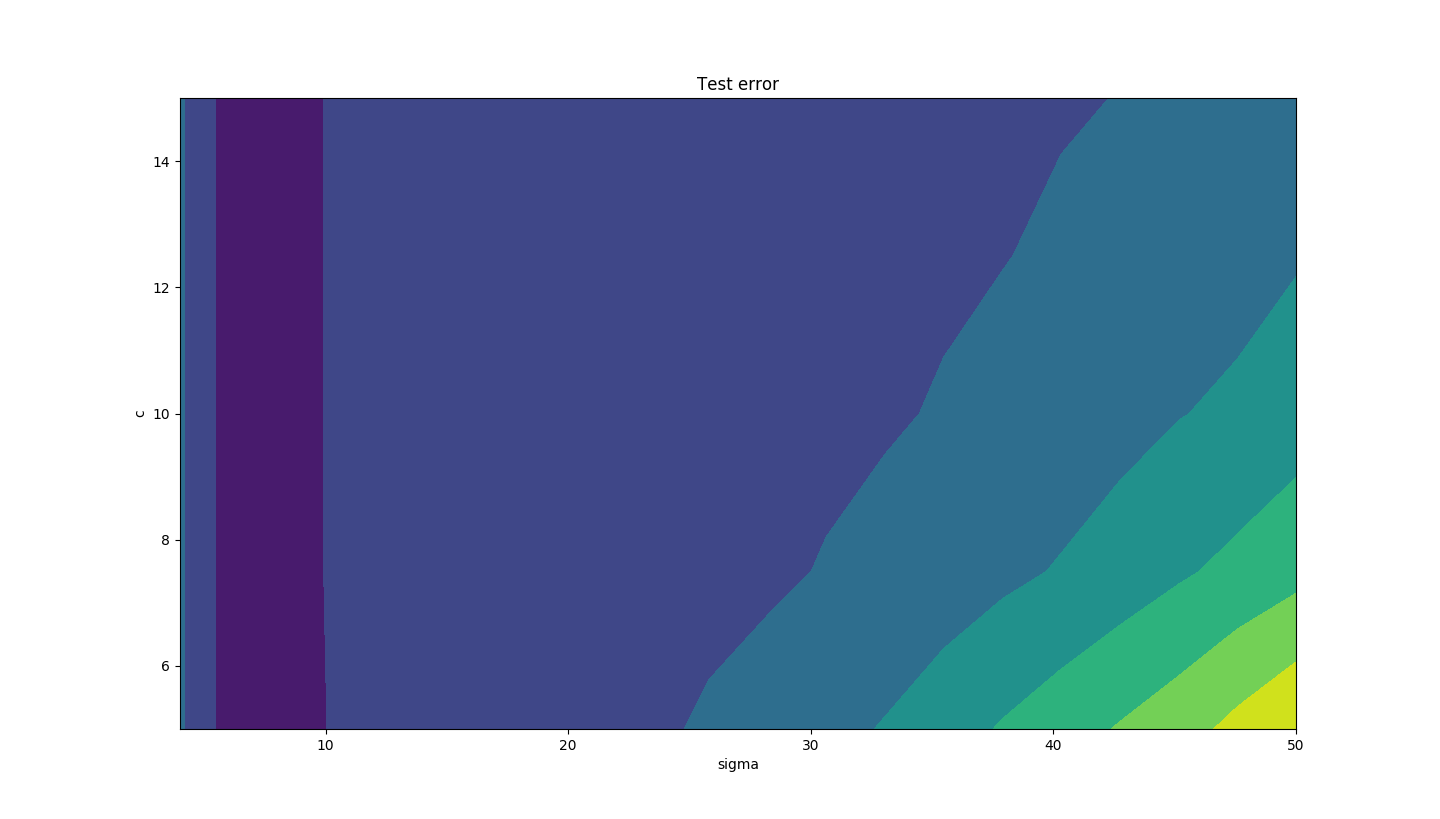
\includegraphics[width=1\textwidth]{figures/new/3_Figure_5}
\end{center}
\caption{\label{fig:3_4}  parameter space of $C$ and $\sigma$  with resulting error  }
\end{figure}



%Best Parameters (c, sigma) = (25.454545454545453, 8.181818181818182) with cv_error = 0.013124320869287314
%continuing...
%RBF-SVM has error = 0.0020408163265306367
%inear-SVM has avg = 0.004081632653061273
%RBF-SVM has avg-error = 0.011227891156462583 min = 0.004081632653061273 max = 0.03367346938775506
%linear-SVM has avg-error = 0.014408163265306122 min = 0.0056122448979591955 max = 0.04081632653061229

%Process finished with exit code 0

